%% Technical report on the first gradient-control campaign (2026-09-26 to 2026-09-27).
%% Build:  latexmk -pdf gclsTechnicalReport.tex      (or: make report-gcls)
%% Every number comes from the archive of the pre-print,
%% ../gcls-level-set-article/data/archive/shared-method-config-2026-09-01-192-g1150e68/,
%% through the same tables and figures (data/tables, data/figures) the pre-print reads, and
%% from STATUS.md section 11 at commit 8867581. Claims carry a mark: MEASURED (a number in the
%% archive), DERIVED (a closed form, re-derived in Appendix B) or HYPOTHESIS (an experiment named).
\documentclass[11pt,a4paper]{article}
\usepackage[a4paper,margin=24mm]{geometry}
\usepackage{amsmath,amssymb}
\usepackage{graphicx}
\usepackage{booktabs}
\usepackage{array}
\usepackage{url}
\makeatletter\g@addto@macro{\UrlBreaks}{\do\-\do\_}\makeatother
\usepackage{siunitx}
\usepackage{caption}
\usepackage[hidelinks]{hyperref}
\graphicspath{{../gcls-level-set-article/data/figures/}}
\newcommand{\tables}{../gcls-level-set-article/data/tables}
\newcommand{\Meas}{\textsc{measured}}
\newcommand{\Der}{\textsc{derived}}
\newcommand{\Hyp}{\textsc{hypothesis}}
\newcommand{\bu}{\mathbf{u}}
\newcommand{\bn}{\mathbf{n}}
\newcommand{\bx}{\mathbf{x}}
\newcommand{\bD}{\mathbf{D}}
\newcommand{\gradh}{\nabla_h}
\newcommand{\per}{\,\si{\per\second}}
\newcommand{\archive}{\path{shared-method-config-2026-09-01-192-g1150e68}}
\setlength{\parskip}{3pt}

\title{Gradient control by source terms and a velocity extension in the leia
semi-Lagrangian level set:\\ why the first campaign failed, and what to do next\\[4pt]
\large Technical report, 2026-09-28}
\author{Prepared by the gradient-control session (Claude Code) for\\
Tomislav Mari\'{c} and Dieter Bothe, Mathematical Modeling and Analysis, TU Darmstadt}
\date{Data: archive \archive; code: commit 8867581, branch \path{feature/gradient-controlled-level-set}}

\begin{document}
\maketitle

\noindent This report is the expert developer's assessment of the first gradient-control
campaign for the supervisor. The pre-print of 2026-09-27 (\path{gclsLevelSet.tex}, the same
theme folder) gives the models, their discretisation and the gate results; this report says
why each candidate failed, which readings of the pre-print it corrects, which routes to abandon
and which to pursue, and in which order. Every claim carries a mark: \Meas{} (a number in the
archive or in STATUS.md, cited), \Der{} (a closed form, re-derived in Appendix~B), or \Hyp{} (an
experiment is named that decides it). The summary comes first; the details follow.

%% ===========================================================================
\section{Summary}
\label{sec:summary}

\paragraph{The verdict in one paragraph.} The six candidates of the first campaign (S1, HL0,
HL1q, HL1z, HL2, FP0) all fail the fixed 2D method gate, and they fail for three reasons that
the pre-print did not name correctly. (i)~The source step is discretised with a centred
gradient of $q=|\nabla\psi|$, a hard band edge and no source-CFL guard; its own map, with no
flow in it, is linearly unstable at a rate of order $\mu$ (\Der, with \Meas{} rates of the
order of $\mu$), and a law that reaches its target puts an $O(1)$ jump of $|\psi|$ at the band
edge (\Der). (ii)~The halo-limited extension at $R=h$ does not remove the normal strain at the
interface; it relocates it into a shell at $d=1$ to $2h$ with a 27\,\% overshoot, inside the
band and the reconstruction stencils (\Der, \Meas{} on the 1D arm). (iii)~The gate has two blind
spots: the exact-1D closed form is undefined for every candidate, so its target criterion is
vacuous, and the centred band-gradient metric cannot see the cell-scale mode that destroyed the
stationary droplet (\Meas{} in the scoring script and the histories). The laws themselves were
never tested, because the discretisation failed first. The next campaign repairs the
discretisation, gates it on a zero-flow static test and on the dossiers' Tier-I cases, and
only then runs a coupled arm.

\paragraph{One line per candidate.}
\begin{center}\small
\begin{tabular}{@{}p{1.1cm}p{3.6cm}p{5.4cm}p{5.2cm}@{}}
\toprule
cand. & what & how it failed (\Meas) & mechanism held responsible (mark) \\
\midrule
S1 & soft wall alone, band $3h$ & shear shape error $411\times$ (order 0.06), gradient target met (0.71); translating $N{=}142$ diverges; oscillating volume error 21; coupled seam 0.76 & the wall's slope reaches $40\sigma$, a bang-bang per-cell map (\Der); the band edge (\Der) \\
HL0 & halo-limited extension, $R=h$ & shear $14\times$, order 1.39, target missed (0.83); oscillating band error $2\times10^7$; translating $64\times$; seam pass & strain relocated into a shell (\Der, \Meas{} 1D); in the coupled arms the sampler injects the spurious current unprojected (\Meas{} translating) or fits across the boundary layer (\Hyp{} oscillating) \\
HL1q & HL0 + linearQ, $\mu=1/T_\mathrm{ref}$ & shear target met (0.20), shape $173\times$ (order 0.02); stationary droplet destroyed at $N{=}200$ (shape $3.8R$, volume 76\,\%); seam pass & the centred-$q$ eigenmode at rate $\sim\mu$ (\Der; rates \Meas); the band edge (\Der) \\
HL1z & HL0 + linearZ & shear band error 10.5, shape 1.65, volume 1.6; stationary destroyed (3.7$R$, 84\,\%); seam pass & as HL1q, plus the unbounded $-\mu q^2/2$ term for large $q$ (\Der) \\
HL2 & HL0 + soft wall & translating diverges at all rungs; oscillating volume error 14.6; shear $400\times$; seam not comparable & S1's and HL0's mechanisms together \\
FP0 & closest-point extension & shear $34\times$ (order 1.38), target missed (0.94); kinematic seam 0.45; coupled seam 1.11; $N{=}200$ runs timed out & no shell, same order loss: the tangential shear of a normal-constant extension and the kinks at the shear tail (\Der); the search is decomposition-dependent (\Meas) \\
\bottomrule
\end{tabular}
\end{center}

\paragraph{Three findings about the baseline bound any candidate.} The curvature of the
moving interface does not converge (2.4 to 3.6\,\% of $1/R$ at every rung of the translating
arm); the oscillating droplet's gradient drift turns unstable at $N=200$ within ten periods
(band gradient error 5.1 at $T$); the translating droplet grows slowly in the interior and fast
near the outlet (all \Meas, STATUS~11.15).

\paragraph{The recommendation.} Abandon as formulated: the halo-limited extension at $R=h$ as a
gradient-control device; HL2; the soft wall as parameterised ($p=5$, $\delta_s=0.08$); FP0 as
a production candidate (keep it as a reference arm); the strain-weight (Taylor, weighted-SDPLS)
route until the curvature-error seed of the spurious current is smaller. Pursue, in this
order: (1)~repair the source discretisation (a one-sided $q$, a smooth band taper, a source-CFL
guard) and gate it on the zero-flow static test and the non-vacuous 1D closed forms; (2)~the
velocity-free linear law on the stationary droplet at $M_\mu\in\{0.1,1,10\}$ with the
prediction ``no growth at a rate of order $\mu$''; (3)~$F$ evaluated at the algebraic foot if
the $O(h)$ crossing shift is still measurable; (4)~the scalar-memory route S2 only after (1) to
(3); (5)~a mesh-resolved extension ($R\ge3h$, the dossier's taper) only for droplets and only if
HL survives the trace test; (6)~V1 last. The experiments, cheapest first, with their
pre-registered predictions are in Table~\ref{tab:experiments}. The rule stands: no candidate
re-enters the coupled gate before the kinematic ladder passes at the baseline's order.

%% ===========================================================================
\section{What was tested and how}
\label{sec:gate}

The fixed 2D method gate (\path{config/gates/methodGate2D.yaml}) runs five arms against the
production method (the baseline): an exact one-dimensional stretch ($u=\alpha x$, closed form
$q=e^{-\alpha t}$; $N=32$ to 256), a reversed shear flow ($N=68$, 96, 136; the kinematic
solver), and a stationary, a translating and an oscillating droplet at the water--air density
ratio ($N=100$, 142, 200; the coupled solver, four MPI ranks). Each arm carries a serial check
of the parallel result. The verdict has four criteria: completion where the baseline completes;
no regression of an error-vector entry by more than 10\,\% beyond the baseline; no observed
order lower than the baseline's by more than 0.3; the target, a band gradient error of the
shear arm at the finest rung at most 0.8 of the baseline's. Table~\ref{tab:cands} lists the
candidates, Table~\ref{tab:verdicts} the verdicts, Table~\ref{tab:seam} the serial checks.
Every number of the campaign is in the archive \archive{} (Appendix~A).

\begin{table}[h]
  \centering\small
  \caption{The candidates of the first campaign (from the pre-print).}
  \label{tab:cands}
  \input{\tables/gcls_candidates.tex}\\[2pt]
  \input{\tables/gcls_candidates_tref.tex}
\end{table}

\begin{table}[h]
  \centering\small
  \caption{Verdicts of the fixed 2D gate. Target ratio: the band gradient error of the shear
  arm at $N=136$ divided by the baseline's (target at most 0.8). The last four columns count the
  failed criteria.}
  \label{tab:verdicts}
  \input{\tables/methodGate2D_verdicts.tex}
\end{table}

\begin{table}[h]
  \centering\small
  \caption{The serial checks: the largest column-scaled difference between one rank and four
  (kinematic arms) or between one rank and four ranks of the coupled translating arm.}
  \label{tab:seam}
  \input{\tables/gcls_gate_seam.tex}
\end{table}

\paragraph{What the dossiers prescribed and the campaign skipped.} The two technical dossiers
that define the direction prescribe Tier-I tests before any coupled run: uniform translation,
rigid rotation, planar strain with $q_0=0.92$, 1.00 and 1.08, and a perturbed scaling. None of
them ran. The zero-flow static test (a signed-distance circle, $u=0$, the source on) did not run
either; it is the cheapest discriminator of Section~\ref{sec:source}.

\paragraph{Two blind spots of the gate (\Meas).} First, the scoring script sets the exact-1D
closed form to \texttt{None} for every candidate that has an extension or a source
(\path{workflow/scripts/make_gate_summary.py}, lines 190 to 198), so \texttt{qError} is
undefined and the target criterion of the 1D arm is vacuous for candidates: the arm can report
a band mean, and it did (Section~\ref{sec:hl}), but it cannot fail anyone. Second, the band
gradient metric of the droplet arms (\texttt{gradPsiMetric leastSquares}, a centred
difference) is blind to a checkerboard: on the stationary droplet at $N=200$ the HL1q curvature
error is $10.6\times$ the baseline's at $t=\SI{4.3}{ms}$ (4.25 against \SI{0.40}{\per\metre})
while the band gradient error is below the baseline's ($3.2\times10^{-4}$ against
$4.4\times10^{-4}$); at \SI{10}{ms} the curvature error is $175\times$ and the band error
$3.9\times$. The kinematic arms carry no curvature column at all. And the soft wall was
inactive on the stationary droplet ($\sigma\approx10^{-3}\per$ and $|q-1|<\delta_s$), so ``S1
equals the baseline to four digits'' there says nothing about its coupled safety.

%% ===========================================================================
\section{The source-term route}
\label{sec:source}

The source step multiplies every cell of the band by $\exp(\Delta t\,F_c)$ after the
characteristic step, with $q_c$ from \texttt{fvc::grad(psi, "gradPsiSource")}, which every case
template sets to \texttt{leastSquares} (a centred gradient), a hard switch at
$|\psi_c|=3h_cq_c$, and a clamp at $|\Delta tF|=30$
(\path{src/leiaLevelSet/semiLagrangian/source/slGradientControlSource.C}, lines 146, 170 and
185 to 194). The law is $F=w(q^2)\,a+G(q^2,\sigma)$ with $w=0$ for every candidate
(\path{gradientControlLaw.H}, lines 182 to 185); \texttt{linearQ} and \texttt{linearZ} have no
$\sigma$. So the linear laws read no velocity. This fact organises the section.

\subsection{The source's own map is linearly unstable with a centred gradient (\Der)}
\label{sec:eigenmode}

Linearise $\psi_c\leftarrow\psi_c\exp(-\mu\Delta t\,(q_c-1))$ about the signed distance
$\psi=d$: with $\psi_c=d_c+\delta_c$ and $q_c\approx1+(\bn\cdot\gradh\delta)_c$,
\begin{equation}
  \delta_c \leftarrow \delta_c-\mu\Delta t\,d_c\,(\bn\cdot\gradh\delta)_c .
  \label{eq:lin}
\end{equation}
For the distance-modulated checkerboard $\delta_c=(-1)^cE\,d_c$ the central difference gives
$(\bn\cdot\gradh\delta)_c=(-1)^{c+1}E$ (Appendix~B), so
$\delta_c\leftarrow\delta_c\,(1+\mu\Delta t)$: an exact eigenmode with growth rate $\mu$,
independent of $\Delta t$, $h$ and the flow; in 2D the mode is $(-1)^{i+j}E\,d$. A one-sided
(Godunov, Rouy--Tourin) $q$ damps the same mode at $2\mu d/h$. A pure checkerboard without the
$d$ modulation is invisible to the centred difference and neutral, which is why the gate's band
metric cannot see the growing mode. Why the stationary droplet exposes it: at $\bu\approx0$ the
semi-Lagrangian step is the identity (\texttt{evaluateRaw} at the cell centre returns $\psi_c$),
so nothing damps the mode; at CFL~0.5 the quadratic fit halves a checkerboard per step, which
hides it in the shear arm. Why SDPLS never saw it: \texttt{R} reads $a$, not $q$, and
\texttt{beta} is \texttt{linearQ} at $\mu=1\per$.

\subsection{The band edge under an accumulated $O(1)$ factor (\Der)}
\label{sec:bandedge}

A law that reaches its target multiplies $|\psi|$ inside the band by
$e^{\int F\,dt}=q_\mathrm{far}/q_\mathrm{target}\approx2$ to 3 in the shear arm and by 1
outside: $|\psi|$ becomes non-monotone at $3h$ (about $7.5h$ inside against $3.5h$ outside),
independent of $h$, and spurious crossings follow. \Meas: HL1z reaches a band error of 10.5 and
a volume error of 1.6 at $T$; HL1q's band error is 0.44 at $t=\SI{1.9}{s}$ and 6.58 at $T$.
With a centred gradient the fixed point ``$q_c=1$ in the band, outside data $c\,d$'' splits
into two sublattices; for $c=1.5$ the odd sublattice's fixed point at the interface cells has
the wrong sign ($\psi(+0.5h)\to-1.25h$), the sign-preserving update drives $|\psi|\to0$ there,
and the zero set moves by $O(0.5h)$ with $\bu=0$. The z-law adds $-\mu q^2/2$, unbounded for the
large $q$ this produces (its runaway at $t\approx0.7$ to \SI{1.0}{s} in the shear arm).

\subsection{HL1q and HL1z on the stationary droplet (\Meas)}
\label{sec:hl1}

The linear laws read no velocity, so the pre-print's loop $\psi\to\kappa\to f\to\bu\to\psi\to
q\to F$ cannot be the primary mechanism. The histories of the archive
(\path{gate/histories_stationary.csv}, $N=200$) show:
\begin{enumerate}
  \item HL1q's curvature error e-folds at about $290\per$ over 10 to \SI{20}{ms} (about
  $460\per$ over 2 to \SI{10}{ms}) and its spurious current at 320 to $350\per$, against
  $\mu=1/T_\mathrm{ref}=270\per$; the mesh-scale capillary rate, $\sqrt{\sigma k^3/\rho}\sim
  10^5\per$, is not seen. The linearised map predicts a rate of exactly $\mu$; the excess is
  not explained (the nonlinear regime, or the flow loop adding to it), and experiment E1.4 (the
  $\mu$ ladder) decides.
  \item HL1q and HL1z agree to three digits until $t=\SI{0.02}{s}$ (curvature error 0.854 and
  0.853 at \SI{2.3}{ms}, 4.25 and 4.24 at \SI{4.3}{ms}, 28.3 and 28.3 at \SI{9.9}{ms}, 484 and
  487 at \SI{19.8}{ms}): their linearisations coincide, and they part only once $|q-1|=O(1)$.
  \item The curvature error leads the velocity: $10.6\times$ the baseline's at \SI{4.3}{ms}
  while the spurious current is $1.4\times$ ($1.05\times10^{-5}$ against
  $7.65\times10^{-6}$\,m/s).
  \item The smooth part of the initial $q$ error decays as the law intends: at \SI{2.3}{ms} the
  band gradient error is $2.2\times10^{-4}$ against the baseline's $4.1\times10^{-4}$.
  \item $\min q$ and $\max q$ leave $[0.99,1.01]$ symmetrically (0.833 and 1.17 at \SI{20}{ms},
  0.329 and 2.29 at \SI{30}{ms}): an oscillatory cell-scale mode, not a smooth drift.
  \item Seed estimate (\Der): the cell-to-cell part of the initial discrete $q$ error is
  $O(h^2/R^2)\approx6\times10^{-4}$ at $N=200$ and reaches $O(1)$ at
  $\ln(1/6\times10^{-4})/270=\SI{27}{ms}$; the droplet is destroyed between 25 and \SI{35}{ms}.
\end{enumerate}
The flow loop is the second stage ($t>\SI{10}{ms}$), once the velocity is slaved to the
curvature error. The clamp at $|\Delta tF|=30$ is never reached (HL1q at $q=190$ has
$\Delta tF=-0.2$); for \texttt{linearQ} $q\to0$ gives $F\to\mu$, bounded, so ``the clamp acts
where $q$ is small'' does not hold.

\subsection{S1: the soft wall is a bang-bang map (\Der{}, \Meas{} seam)}
\label{sec:s1}

The slope of the soft wall $G=-C_\kappa\sigma\,\mathrm{sign}(e)\tanh(\gamma(|e|/\delta_s)^p)$,
$e=q-1$, at $C_\kappa=1.25$, $\delta_s=0.08$, $p=5$, $\gamma=\mathrm{artanh}\,0.9$ reaches
$|dG/dq|=40.3\,\sigma$ at $|e|=0.069$ (Appendix~B), so $\Delta t\,dG/dq\approx0.5$ per step in
the shear arm ($\sigma\approx3\per$, $\Delta t=\SI{4.1e-3}{s}$): a nearly discontinuous
per-cell map. Its signature is the 76\,\% seam failure of S1; HL1q and HL1z pass the same check
at $4.9\times10^{-7}$ and $5.3\times10^{-7}$, so ``round-off in $q_c$ carried into $F$'' is not
their mechanism. In the coupled arms the wall reads $\sigma$ of the spurious current: that, and
only that, is the SDPLS loop of the pre-print. The 1D arm shows the same map failing under
refinement: S1's band mean goes 0.998, 0.926, 0.746, 0.697 at $N=32$ to 256 instead of
converging to the continuum fixed point (\Meas).

\subsection{What the pre-print's mechanisms explain, and what they do not}
\label{sec:preprint}

The crossing shift $\delta=h\,ab/(a+b)^2\,\Delta t\,(F_A-F_B)$ is first order in $h$: for the
linear laws $F_A-F_B=-\mu(q_A-q_B)$, and summed over the shear run $|\delta|\le(h/4)\,\mu T
\max|\Delta q|\approx0.2h$ (\Der). The measured HL1q shape error of 0.107 at $N=136$ is a
$\sim1.1h$ radial displacement of the whole perimeter, with an order of 0.02, flat in $N$
(0.108, 0.117, 0.107); S1's 0.265, 0.327, 0.254 is flat too. An $O(h)$ mechanism cannot produce
an $O(1)$ error, so the shift is a secondary contribution; the band edge of
Section~\ref{sec:bandedge} is the $O(1)$ one. The band-edge kink at $3h$ lies outside the
interface cells' CPC stencils (reach about $2.4h$), so it reaches the interface through the
source's own dynamics and through transport, not through the fit of the interface cells. The
normal-projected-SL result (a per-cell write-back keyed on the \emph{fitted} gradient has $O(1)$
noise gain) does not transfer directly: the source reads \texttt{fvc::grad}, not the fit.

%% ===========================================================================
\section{The velocity-extension route}
\label{sec:hl}

\subsection{$R=h$ relocates the normal strain; it does not remove it (\Der, \Meas)}
\label{sec:relocation}

For travel \texttt{capped} with $m=2$ and weight \texttt{fractionReached} with $\beta=1$ the
extension samples at $Y=\bx-S\bn$ with $S=c\,d$ and blends with $w=c$,
$c=(1+t^4)^{-1/4}$, $t=d/R$. Linearised, $\bu_H=\bu-wS\,\partial_n\bu$, and the normal strain it
transmits at $d=tR$ is (Appendix~B)
\begin{equation}
  K(t)=1-\frac{d(wS)}{dd}=1-(1-t^4)(1+t^4)^{-3/2}
  =0,\;0.14,\;1.00,\;1.27,\;1.21,\;1.11\quad\text{at }t=0,\,0.5,\,1,\,1.5,\,2,\,3,
\end{equation}
with $\int_0^D(1-K)\,dd=wS(D)\to R^2/D$. The strain is displaced by about $1.5h$ into a shell
with a 27\,\% overshoot, not removed, and with $R=h$ the shell sits inside the
geometry-evaluation neighbourhood (band $3h$, stencil $1.4h$), which the dossier itself forbids
(``the transition should be broad, located outside the geometry-evaluation neighbourhood'').
The 1D arm measures it: HL0's band mean $q$ is 0.589, 0.499, 0.510, 0.459 at $N=32$ to 256,
against $e^{-1}=0.368$ for the baseline at every rung, 0.99 to 1.09 for FP0, and 0.49 for the
band average of $e^{-K}$ over $d=0.5h$, $1.5h$, $2.5h$. In the shear arm at $t=\SI{0.02}{s}$
(five steps) the band error is 0.0200 for HL0, 0.0354 for the baseline and 0.0005 for FP0. The
pre-registered HL0 read-out (``zero normal strain on the interface, so the band error falls'')
conflated the interface with the band. The $q$ profile then varies by $O(1)$ over one cell
($\psi'''\sim0.6/h^2$), so the quadratic reconstruction error at the feet is $\sim0.1h$ instead
of $\sim4\times10^{-4}h$: first-order transport whatever the trace velocity (\Der). The
HL0/baseline shape-error ratio grows $4.3$, $8.4$, $13.7$ over the three shear rungs (orders
1.39 against 3.07, \Meas).

\subsection{The reconstruct argument is neither necessary nor sufficient (\Meas)}

The pre-print blamed the face-to-cell reconstruction of a flux correction that varies within a
cell. FP0 has no shell (\texttt{phiExt = interpolate(Uext)\,.\,Sf}, smooth on the flow scale)
and loses the same order, 1.38: within-cell variation is not necessary. HL0's excess volume
error ($2.3\times10^{-4}$ against $5.5\times10^{-5}$) appears by $t=\SI{0.02}{s}$, before any
$q$ kink exists: the shell is not sufficient for the early error either. The reconstruction is
one $O(h|\nabla\bu|)$ contribution among others.

\subsection{The coupled arms: unprojected injection and the boundary layer}

The translating droplet has no physical gradient to fit across (rigid translation, $\bD=0$),
and HL0 fails $64\times$ there (order $-3.1$). What the sampler reads is the cell-scale
spurious current $u'$ ($\sim6\times10^{-4}$\,m/s), and the extension injects
$w[\bu_h(Y)-\bu_h(\bx)]\sim u'$ into the trace flux unprojected, while the baseline traces
\texttt{reconstruct(phi)}, the smoothest velocity the solver has. \Meas: HL0 tracks the
baseline to $t\approx\SI{0.02}{s}$ (curvature error 77 against \SI{67}{\per\metre}), then its
curvature error and velocity grow together at about 235 and $210\per$ over 30 to \SI{45}{ms},
while the baseline stays near \SI{35}{\per\metre} and $6\times10^{-4}$\,m/s. The oscillating
droplet is where the pre-print's sampler-across-the-jump reading is plausible (\Hyp): the
air-side boundary layer $\delta\approx\sqrt{\nu_\mathrm{air}T}\approx8h$ at $N=200$ gives
$\partial_nu_t\approx250\per$, the fit across the kink extrapolates the water side by up to
$25\times$, and HL0's band gradient error grows at about $480\per$ over 10 to \SI{20}{ms} (0.29
to 29.5), five times the physical strain. The sample point $Y_f$ can lie $1.5h$ from a cell
centre, outside the $3\times3$ hull (\texttt{evaluateRaw} has no trust region). The ratio-1 test
of the pre-print cannot separate the two readings (it shrinks $u'$ and the kink at once);
sampling \texttt{reconstruct(phi)} instead of \texttt{U} can (E1.6).

\subsection{FP0, and what every normal-constant extension does to the band}

FP0 has no shell, loses the same order, is seam-dependent (0.45 kinematic: the closest-point
search depends on the decomposition at the processor boundaries; 1.11 coupled), and collapses at
the shear tail (band error 0.001 to 0.03 until $t=\SI{0.1}{s}$, 0.66 by \SI{0.4}{s} with a
volume error of $3.6\times10^{-2}$; the search fails at the tail and the distance function's
kinks come within $3h$). Any velocity constant along the normals shears the band tangentially:
level sets at distance $d$ from a circle of radius $R$ rotate at $\Omega(d)=\omega R/(R+d)$
(closest point) or $\omega(R+d(1-c^2))/(R+d)$ (halo-limited); a circle is invariant, a slotted
disc is not (\Der; the Tier-I rigid-rotation test decides). The baseline avoids both by
transporting a smooth, non-distance $\psi$ at third order.

\subsection{Two more facts of the implementation}

The extension geometry ($d$, $\mathbf e$, $w$, $S$, $Y$) is evaluated before the $\psi^n$
restore of the outer loop (\path{slAlphaEqn.H}, \texttt{slVelExt->correct()} at line 71, the
restore at line 149), so on outer passes 2 and 3 it comes from $\psi^{n+1,(k-1)}$ while $\psi^n$
is transported; with $R=h$ a CFL$\cdot h$ shift in $d$ changes $w$ by up to 0.3 ($w=0.84$ at
$h$, 0.50 at $2h$). Coupled solver only; E1.5 decides whether it matters. And the $R$ ladder
the pre-print proposed is blocked by construction: \texttt{radiusCells > 1} is a
\texttt{FatalIOError} (\path{haloLimited.C}, lines 108 to 114), because the sampler evaluates
the face's own cells' models; $R=2$ to $3h$ needs a sampler that locates the cell containing
$Y$ with a 2 to 3 layer halo, the halo the design set out to avoid. Checked and consistent: the
AB2 foot with \texttt{UextOld}, the departure-centred form, the physical patch values, and the
source's time level.

\begin{figure}[t]
  \centering
  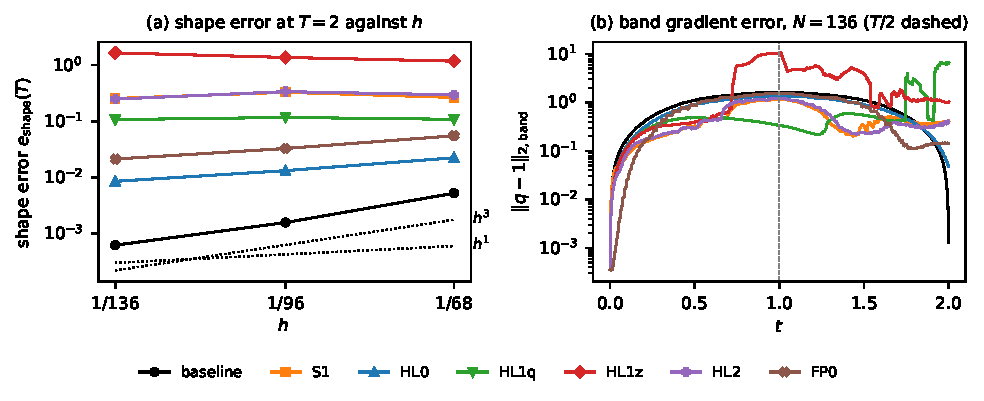
\includegraphics[width=\textwidth]{gcls_shear.pdf}
  \caption{The reversed shear flow (from the pre-print). (a) The shape error at $T$ against
  $h$; the dotted lines show the slopes one and three. (b) The band gradient error at $N=136$
  over time.}
\end{figure}
\begin{figure}[t]
  \centering
  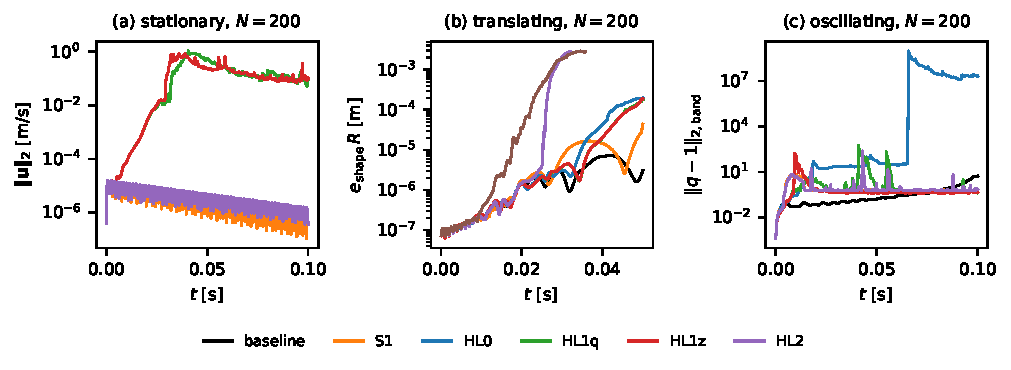
\includegraphics[width=\textwidth]{gcls_droplets.pdf}
  \caption{The droplet arms at $N=200$ (from the pre-print): (a) the spurious current of the
  stationary droplet, (b) the shape error of the translating droplet, (c) the band gradient
  error of the oscillating droplet.}
\end{figure}

%% ===========================================================================
\section{The baseline's own limits, and the gate's blind spots as repairs}
\label{sec:baseline}

Three results of the baseline bound what any candidate can show (\Meas, STATUS~11.15): the
curvature of the moving interface does not converge (2.4 to 3.6\,\% of $1/R$ at every rung of
the translating arm, while the same estimator converges at order 1.9 on the stationary droplet);
the gradient drift of the oscillating droplet turns unstable at $N=200$ within ten periods, so
the finest rung of that arm cannot carry a verdict, and it is the case on which a working
candidate must first show a gain; the translating droplet grows slowly in the interior (about
$30\per$ from \SI{0.10}{s} in a \SI{20}{mm} box) and fast near the outlet, so a horizon beyond
\SI{0.05}{s} needs a longer box. The gate repairs that follow from Section~\ref{sec:gate}:
the candidates' closed forms in the 1D arm (E0.1); a checkerboard-sensitive band diagnostic (the
$L^2$ norm of the second difference of $\psi$, or $\min$ and $\max$ of a one-sided $q$); a
curvature column in the kinematic arms; the zero-flow static arm; and the extension's time level
on outer passes $\ge2$ (move \texttt{slVelExt->correct()} after the restore, or document it).

%% ===========================================================================
\section{Assessment and recommendation}
\label{sec:assessment}

\paragraph{Abandon as formulated.} The halo-limited extension at $R=h$ as a gradient-control
device (Section~\ref{sec:relocation}: it cannot protect the band, and enlarging $R$ makes it
FP-like in halo cost). HL2. The soft wall as parameterised ($p=5$, $\delta_s=0.08$ is
bang-bang, seam-amplifying, and ``safe'' on the stationary droplet only because it was off; it
reads $\sigma$ of the spurious current, the SDPLS loop). FP0 as a production candidate
(seam-dependent, collapses at the shear tail; keep as a reference arm). The Taylor/weighted-SDPLS
strain route: the dossier states it is weighted SDPLS at the PDE level, and SDPLS~\texttt{R}
failed under coupling through the $a$-reading loop with a curvature-error seed the force side
owns; a weight $w\le1$ reduces that gain by at most $w$, and $w=1$ in the geometry cells by
design.

\paragraph{Pursue, in order.}
\begin{enumerate}
  \item Repair the source discretisation before testing any law: a one-sided (Rouy--Tourin) $q$
  on unstructured meshes, $q_c=\max_{N:\,|\psi_N|<|\psi_c|}(|\psi_c|-|\psi_N|)/|\bx_N-\bx_c|$
  over the face neighbours including the coupled-patch neighbours (E2.1); a smooth band taper
  $F\,\tau(|\psi|/(3hq))$ with a $C^2$ cutoff, or no band (E2.2); a source-CFL guard
  $\mu\,3h\,\Delta t/h<1/2$. Verify with E1.1 to E1.3 and the non-vacuous 1D closed forms
  (E0.1). Then the stationary droplet at $M_\mu\in\{0.1,1,10\}$ is the first coupled gate, with
  the prediction ``no growth at a rate of order $\mu$''; a slower residual growth is the
  force-side seed of the SDPLS paper, and no source fixes it.
  \item The velocity-free linear law (\texttt{linearQ}, strain weight \texttt{none}) as the
  only family with a clean linearisation. Its offset $q^*=1-a/\mu$ means $\mu\approx10/T_\mathrm{ref}$
  in strained arms, which is exactly why the discretisation must be monotone first.
  \item $F$ evaluated at the algebraic foot $\bx_c-d\,\bn$ and copied along the normal (E2.4),
  if the $O(h)$ crossing shift is still measurable after (1).
  \item S2 (a scalar memory $Q$ that filters $q$) only after (1) to (3), in the variant that
  relaxes to the one-sided $q_h$ (otherwise it inherits the eigenmode), and with its
  $a_h/\sigma_h$ term off first, because that term re-enters the SDPLS loop.
  \item ALG (the uncapped algebraic sample, $w=1$ in the band, the dossier's $K$ taper with
  $\ell_0=3h$, $\ell_1=6h$, $K_p\approx1.8$) only if an extension is still wanted for droplets:
  it is the honest HL with $R\ge$ band width and a 3 to 6 layer halo, and it does not help the
  vortex.
  \item V1 last, and only if (1) to (4) fail for lack of orientation memory (the dossier's own
  rule).
\end{enumerate}

\begin{table}[p]
  \centering\small
  \caption{The experiment ladder, cheapest first. Each prediction is written before its run.}
  \label{tab:experiments}
  \begin{tabular}{@{}p{1.3cm}p{5.0cm}p{5.0cm}p{3.6cm}@{}}
  \toprule
  id (cost) & experiment & prediction & it falsifies \\
  \midrule
  E0.1 (hours) & candidate closed forms in the 1D arm: $\dot q=q(F-\alpha K(d/R))$, $\dot d=\alpha d(1-c^2)$ per band cell & HL0 band mean $\approx0.49$ (measured 0.46 to 0.59); S1 $\to0.925$ (measured $0.998\to0.697$); HL1q with $\mu=\alpha$: band mean $\to\sim0.5$ (measured $0.80\to0.53$) & nothing yet; it makes the 1D gate real \\
  E1.1 (dict.) & zero-flow static test: kinematic solver, $\bu=0$, circle SDF, $N=100$, \texttt{linearQ}, band $3h$, $\mu\in\{27,270,2700\}\per$, $\mu\Delta t\le10^{-2}$ & $\max|\psi_c-d_c|$ grows as $e^{\mu t}$ with the pattern $(-1)^{i+j}d$; the fit curvature error grows at $\mu$; the centred metric stays $O(\text{seed})$ until the amplitude is $O(h)$; rates 1:10:100 & mechanism A; if nothing grows at $\bu=0$ the source map is stable and the flow-loop reading returns \\
  E1.2 & E1.1 with $\psi_0=1.5d$ (dossier B1, Tier-I test 4) & $|\psi|\to0$ in the interface cells on one sublattice within $\sim5/\mu$; zero-set displacement $O(0.5h)$; $c=1.08$: 0.1 to $0.2h$ & mechanism B, if the zero set stays put to $O(h^2)$ \\
  E1.3 & E1.1 and E1.2 with band 1000 cells & B disappears, A remains & separates A from B \\
  E1.4 & HL1q stationary at $M_\mu=0.1$ and 10 & survives \SI{0.1}{s} / dies by $\sim$\SI{3.5}{ms}; rate $\propto\mu$ & A as the primary mechanism \\
  E1.5 & HL0 translating with \texttt{psiOuterCorrectors no} & the departure from the baseline moves later or vanishes if the time-level mismatch matters & the time-level mismatch \\
  E1.6 & HL0 translating and oscillating with the extension sampling \texttt{reconstruct(phi)} instead of \texttt{U} & translating improves, oscillating does not; then ratio 1 for the oscillating arm & unprojected injection against the jump reading \\
  E1.7 & S1 with $\delta_s=0.3$, $p=1$ (slope $\approx6\sigma$) & seam $\le10^{-5}$, shear shape error $\ge10\times$ lower, band-error gain shrinks & the bang-bang reading, if the seam still fails \\
  E2.1 (days) & upwind $q$ in the source, plus the source-CFL guard & E1.1's mode damped at $2\mu d/h$; HL1q stationary at the baseline level for \SI{0.1}{s} & A \\
  E2.2 & smooth band taper, or no band & HL1q and S1 shear shape orders rise from $\sim0$ to $\ge1$ & B \\
  E2.3 & kinematic \texttt{cellCentred} trace with $\bu_\mathrm{ext}$ (\path{leiaSemiLagrangeLevelSetFoam.C}, line 218) & the HL0 shear constant drops, the order stays $<2$ (the shell remains); order 3 would mean the trace alone was the cause & the relocation reading \\
  E2.4 & $F$ at the algebraic foot, copied along the normal & the $O(h)$ shift vanishes at first order; A and B remain unless E2.1 and E2.2 & the crossing-shift contribution \\
  E3 (weeks) & extended sampler with \texttt{findCell} and a 3-layer halo for $R=3h$; S2 & only if HL survives E2.3 & --- \\
  \bottomrule
  \end{tabular}
\end{table}

%% ===========================================================================
\appendix
\section{Data and reproducibility}
\label{app:data}

Every number of this report comes from the archive
\path{docs/gradient-controlled-level-set/gcls-level-set-article/data/archive/}\archive{}
(README.md, MANIFEST.csv with SHA-256): the fixed gate (\path{gate/}: the summaries, verdicts,
orders, seam checks and reduced histories of every arm), the pre-fix gate (\path{prefix/}) and
the laptop discriminators (\path{laptop/}), and from STATUS.md section~11 at commit 8867581.
The growth rates of Sections~\ref{sec:hl1} and~\ref{sec:hl} are least-squares slopes of
$\ln(\text{value})$ against time over the stated windows of
\path{gate/histories_stationary.csv}, \path{histories_translating.csv} and
\path{histories_oscillating.csv}; the band means of the 1D arm are the \texttt{qBandMean}
column of \path{gate/summaries/<candidate>/summary.csv}. The candidate configurations with their
pre-registered read-outs are \path{config/candidates/*.yaml}; the gate is
\path{config/gates/methodGate2D.yaml}; the tables are those of the pre-print
(\path{data/tables/}). Code: \path{src/leiaLevelSet/gradientControl/} (the laws),
\path{src/leiaLevelSet/semiLagrangian/source/} (the source step),
\path{src/leiaLevelSet/velocityExtension/haloLimited/} (the extension),
\path{applications/solvers/leiaSemiLagrangianLevelSetTwoPhaseFoam/slAlphaEqn.H} (the outer
loop), \path{workflow/scripts/make_gate_summary.py} (the scoring).

\section{Derivations}
\label{app:derivations}

\paragraph{The transmitted strain of the capped, fraction-reached extension.} With
$t=d/R$, $c=(1+t^4)^{-1/4}$, $S=c\,d$ and $w=S/d=c$, the linearised extension is
$\bu_H=(1-w)\bu+w\,\bu(\bx-S\bn)=\bu-wS\,\partial_n\bu+O(S^2)$. For a normal strain that is
uniform across the shell, $\partial_n\bu_H=\partial_n\bu\,[1-d(wS)/dd]$, and with
$wS=c^2d=d(1+t^4)^{-1/2}$,
\[
  \frac{d(wS)}{dd}=(1+t^4)^{-1/2}-2t^4(1+t^4)^{-3/2}=(1-t^4)(1+t^4)^{-3/2},
  \qquad K(t)=1-(1-t^4)(1+t^4)^{-3/2}.
\]
$K(0)=0$, $K(1)=1$, $K(1.5)=1+4.0625\cdot6.0625^{-3/2}=1.272$, $K(2)=1.214$, $K(3)=1.108$,
$K\to1$ from above. $\int_0^D(1-K)\,dd=wS(D)=D(1+(D/R)^4)^{-1/2}\to R^2/D$ for $D\gg R$: the
removed strain integrates to zero over the band, so the extension displaces it. (The dossier's
identity $K=1-w-sw'$ and its overshoot proposition concern the uncapped sample; the capped
version has two strain-transmitting factors and the same conserved integral.)

\paragraph{The checkerboard eigenmode of the centred exponential source.} From
Eq.~\eqref{eq:lin} in one dimension with the central difference
$(\bn\cdot\gradh\delta)_c=(\delta_{c+1}-\delta_{c-1})/(2h)$ and $\delta_c=(-1)^cE\,d_c$,
$d_{c\pm1}=d_c\pm h$:
$\delta_{c+1}-\delta_{c-1}=-(-1)^cE[(d_c+h)-(d_c-h)]=-2h(-1)^cE$, so
$(\bn\cdot\gradh\delta)_c=(-1)^{c+1}E$ and
$\delta_c\leftarrow(-1)^cE\,d_c+\mu\Delta t\,d_c(-1)^cE=\delta_c(1+\mu\Delta t)$. With the
one-sided difference towards the interface, $(\delta_c-\delta_{c-1})/h=(-1)^cE(2d_c-h)/h$, and
$\delta_c\leftarrow\delta_c[1-\mu\Delta t(2d_c-h)/h]\approx\delta_c(1-2\mu\Delta t\,d_c/h)$:
damped at $2\mu d/h$. In two dimensions the mode $(-1)^{i+j}E\,d$ gives the same rate $\mu$ for
the least-squares gradient projected on $\bn$; a one-dimensional checkerboard $(-1)^iE\,d$ grows
at $\mu n_x^2\le\mu$.

\paragraph{The soft-wall slope.} $G=-C_\kappa\sigma\,\mathrm{sign}(e)\tanh(\gamma x)$ with
$x=(|e|/\delta_s)^p$; $|dG/de|=C_\kappa\sigma\,\gamma p\,(|e|/\delta_s)^{p-1}\delta_s^{-1}
\operatorname{sech}^2(\gamma x)$. Its maximum over $e$ at $C_\kappa=1.25$, $\delta_s=0.08$,
$p=5$, $\gamma=\mathrm{artanh}\,0.9=1.472$ is $40.3\,\sigma$ at $|e|=0.069=0.86\,\delta_s$
(numerically); with $\sigma=3\per$ and $\Delta t=\SI{4.1e-3}{s}$, $\Delta t\,|dG/de|=0.50$.

\paragraph{The summed crossing shift.} $ab/(a+b)^2\le1/4$, so over $n$ steps
$|\delta_\mathrm{total}|\le(h/4)\sum_n\Delta t\,|F_A-F_B|\le(h/4)\,\mu T\max|q_A-q_B|$; with
$\mu T=2$ and $|\Delta q|\le0.4$ in the shear arm, $|\delta_\mathrm{total}|\le0.2h$.

\end{document}
